\documentclass{article}\usepackage[]{graphicx}\usepackage[]{color}
%% maxwidth is the original width if it is less than linewidth
%% otherwise use linewidth (to make sure the graphics do not exceed the margin)
\makeatletter
\def\maxwidth{ %
  \ifdim\Gin@nat@width>\linewidth
    \linewidth
  \else
    \Gin@nat@width
  \fi
}
\makeatother

\definecolor{fgcolor}{rgb}{0.345, 0.345, 0.345}
\newcommand{\hlnum}[1]{\textcolor[rgb]{0.686,0.059,0.569}{#1}}%
\newcommand{\hlstr}[1]{\textcolor[rgb]{0.192,0.494,0.8}{#1}}%
\newcommand{\hlcom}[1]{\textcolor[rgb]{0.678,0.584,0.686}{\textit{#1}}}%
\newcommand{\hlopt}[1]{\textcolor[rgb]{0,0,0}{#1}}%
\newcommand{\hlstd}[1]{\textcolor[rgb]{0.345,0.345,0.345}{#1}}%
\newcommand{\hlkwa}[1]{\textcolor[rgb]{0.161,0.373,0.58}{\textbf{#1}}}%
\newcommand{\hlkwb}[1]{\textcolor[rgb]{0.69,0.353,0.396}{#1}}%
\newcommand{\hlkwc}[1]{\textcolor[rgb]{0.333,0.667,0.333}{#1}}%
\newcommand{\hlkwd}[1]{\textcolor[rgb]{0.737,0.353,0.396}{\textbf{#1}}}%
\let\hlipl\hlkwb

\usepackage{framed}
\makeatletter
\newenvironment{kframe}{%
 \def\at@end@of@kframe{}%
 \ifinner\ifhmode%
  \def\at@end@of@kframe{\end{minipage}}%
  \begin{minipage}{\columnwidth}%
 \fi\fi%
 \def\FrameCommand##1{\hskip\@totalleftmargin \hskip-\fboxsep
 \colorbox{shadecolor}{##1}\hskip-\fboxsep
     % There is no \\@totalrightmargin, so:
     \hskip-\linewidth \hskip-\@totalleftmargin \hskip\columnwidth}%
 \MakeFramed {\advance\hsize-\width
   \@totalleftmargin\z@ \linewidth\hsize
   \@setminipage}}%
 {\par\unskip\endMakeFramed%
 \at@end@of@kframe}
\makeatother

\definecolor{shadecolor}{rgb}{.97, .97, .97}
\definecolor{messagecolor}{rgb}{0, 0, 0}
\definecolor{warningcolor}{rgb}{1, 0, 1}
\definecolor{errorcolor}{rgb}{1, 0, 0}
\newenvironment{knitrout}{}{} % an empty environment to be redefined in TeX

\usepackage{alltt}

% \usepackage[utf8]{inputenc}
\usepackage{amsmath}
\usepackage{fancyhdr}
\usepackage{array}
\usepackage{longtable}
\usepackage{graphicx}
\usepackage{color}
\usepackage[letterpaper, margin=1in]{geometry}
\usepackage{lscape}
\newcommand{\blandscape}{\begin{landscape}}
\newcommand{\elandscape}{\end{landscape}}
\usepackage{dcolumn}
\usepackage{bbm}
\usepackage{threeparttable}
\usepackage{booktabs}
\usepackage{expex}
\usepackage{pdflscape}
\usepackage{rotating, graphicx}
\usepackage{tabulary}
\usepackage{lscape}
\usepackage{makecell}
\usepackage{algorithm}
\usepackage{multirow}
\usepackage{colortbl}
\usepackage{longtable}
\usepackage{array}
\usepackage{multirow}
\usepackage{wrapfig}
\usepackage{float}
\usepackage{pdflscape}
\usepackage{tabu}
\usepackage{threeparttable}

\title{%
Homework 9\\
\large Applied Mutlivariate Analysis}
\date{November 1, 2018}
\author{Emorie Beck}
\IfFileExists{upquote.sty}{\usepackage{upquote}}{}
\begin{document}
\maketitle
% \SweaveOpts{concordance=TRUE}

\section{Workspace}
\subsection{Packages}



\begin{knitrout}
\definecolor{shadecolor}{rgb}{0.969, 0.969, 0.969}\color{fgcolor}\begin{kframe}
\begin{alltt}
\hlkwd{library}\hlstd{(car)}
\hlkwd{library}\hlstd{(knitr)}
\hlkwd{library}\hlstd{(psych)}
\hlkwd{library}\hlstd{(gridExtra)}
\hlkwd{library}\hlstd{(knitr)}
\hlkwd{library}\hlstd{(kableExtra)}
\hlkwd{library}\hlstd{(MASS)}
\hlkwd{library}\hlstd{(vegan)}
\hlkwd{library}\hlstd{(smacof)}
\hlkwd{library}\hlstd{(scatterplot3d)}
\hlkwd{library}\hlstd{(ape)}
\hlkwd{library}\hlstd{(ade4)}
\hlkwd{library}\hlstd{(ecodist)}
\hlkwd{library}\hlstd{(cluster)}
\hlkwd{library}\hlstd{(factoextra)}
\hlkwd{library}\hlstd{(candisc)}
\hlkwd{library}\hlstd{(ggdendro)}
\hlkwd{library}\hlstd{(lme4)}
\hlkwd{library}\hlstd{(plyr)}
\hlkwd{library}\hlstd{(tidyverse)}
\end{alltt}
\end{kframe}
\end{knitrout}



\subsection{data}
The file, Set\_8.csv, contains the data from a follow-up to the job search study. The file contains GRE scores (Verbal + Quantitative) upon entering graduate school, number of publications while in graduate school, length of time to complete the Ph.D. (in years), and the outcome of the job search (1=no interviews, 2=got a job, 3=interviews but no job). The variable, sample, divides the sample into two random halves. Analyze the data from sample=1 using discriminant analysis to determine how best to predict job search outcome. Use sample=2 for cross- validation. Answer the following questions.

\begin{knitrout}
\definecolor{shadecolor}{rgb}{0.969, 0.969, 0.969}\color{fgcolor}\begin{kframe}
\begin{alltt}
\hlstd{wd} \hlkwb{<-} \hlstr{"https://github.com/emoriebeck/homeworks/raw/master/multivariate/homeworks/homework10"}

\hlstd{dat} \hlkwb{<-} \hlkwd{sprintf}\hlstd{(}\hlstr{"%s/Set_8.csv"}\hlstd{, wd)} \hlopt \hlkwd{read.csv}\hlstd{(.,} \hlkwc{stringsAsFactors} \hlstd{= F)}

\hlstd{dat1} \hlkwb{<-} \hlstd{dat} \hlopt \hlkwd{filter}\hlstd{(sample} \hlopt{==} \hlnum{1}\hlstd{)}
\hlstd{dat2} \hlkwb{<-} \hlstd{dat} \hlopt \hlkwd{filter}\hlstd{(sample} \hlopt{==} \hlnum{2}\hlstd{)}
\end{alltt}
\end{kframe}
\end{knitrout}


\section{Question 1}
How many discriminant functions are significant?

\begin{knitrout}
\definecolor{shadecolor}{rgb}{0.969, 0.969, 0.969}\color{fgcolor}\begin{kframe}
\begin{alltt}
\hlcom{# lda}
\hlstd{LDA_1} \hlkwb{<-} \hlkwd{lda}\hlstd{(outcome} \hlopt{~} \hlstd{gre} \hlopt{+} \hlstd{pubs} \hlopt{+} \hlstd{years,}  \hlkwc{data} \hlstd{= dat1)}

\hlcom{# cda}
\hlstd{MLM_1} \hlkwb{<-} \hlkwd{lm}\hlstd{(}\hlkwd{cbind}\hlstd{(gre, pubs, years)}\hlopt{~}\hlkwd{as.factor}\hlstd{(outcome),}\hlkwc{data}\hlstd{=dat1)}
\hlstd{CDA_1} \hlkwb{<-} \hlkwd{candisc}\hlstd{(MLM_1,} \hlkwc{data}\hlstd{=dat1)}

\hlstd{CDA_1}
\end{alltt}
\begin{verbatim}
## 
## Canonical Discriminant Analysis for as.factor(outcome):
## 
##     CanRsq Eigenvalue Difference Percent Cumulative
## 1 0.791158   3.788299     3.6939 97.5698      97.57
## 2 0.086221   0.094356     3.6939  2.4302     100.00
## 
## Test of H0: The canonical correlations in the 
## current row and all that follow are zero
## 
##   LR test stat approx F numDF denDF   Pr(> F)    
## 1      0.19084   105.28     6   490 < 2.2e-16 ***
## 2      0.91378              2                    
## ---
## Signif. codes:  0 '***' 0.001 '**' 0.01 '*' 0.05 '.' 0.1 ' ' 1
\end{verbatim}
\end{kframe}
\end{knitrout}

One discriminant function is significant.

\section{Question 2}
Comment on the irrelative "importance."

There is only one function, so it is all that is important.

\section{Question 3}
How would you interpret the(se) function(s)?

\begin{knitrout}
\definecolor{shadecolor}{rgb}{0.969, 0.969, 0.969}\color{fgcolor}\begin{kframe}
\begin{alltt}
\hlstd{LDA_Values} \hlkwb{<-} \hlkwd{predict}\hlstd{(LDA_1)}
\hlkwd{as.data.frame}\hlstd{(LDA_Values}\hlopt{$}\hlstd{x)} \hlopt
  \hlkwd{bind_cols}\hlstd{(}\hlkwd{data.frame}\hlstd{(}\hlkwc{class} \hlstd{= LDA_Values}\hlopt{$}\hlstd{class))} \hlopt
  \hlkwd{group_by}\hlstd{(class)} \hlopt
  \hlkwd{summarize_at}\hlstd{(}\hlkwd{vars}\hlstd{(}\hlopt{-}\hlstd{class),} \hlkwd{funs}\hlstd{(mean),} \hlkwc{na.rm} \hlstd{= T)}
\end{alltt}
\begin{verbatim}
## # A tibble: 3 x 3
##   class    LD1    LD2
##   <fct>  <dbl>  <dbl>
## 1 1     -3.53  -0.213
## 2 2      2.42  -0.479
## 3 3      0.307  0.292
\end{verbatim}
\begin{alltt}
\hlkwd{as.data.frame}\hlstd{(LDA_Values}\hlopt{$}\hlstd{x)} \hlopt
  \hlkwd{bind_cols}\hlstd{(}\hlkwd{data.frame}\hlstd{(}\hlkwc{Class} \hlstd{= LDA_Values}\hlopt{$}\hlstd{class))} \hlopt
  \hlkwd{gather}\hlstd{(}\hlkwc{key} \hlstd{= Function,} \hlkwc{value} \hlstd{= Score,} \hlopt{-}\hlstd{Class)} \hlopt
  \hlkwd{mutate}\hlstd{(}\hlkwc{Class_long} \hlstd{=} \hlkwd{mapvalues}\hlstd{(Class,} \hlkwc{from} \hlstd{=} \hlkwd{c}\hlstd{(}\hlnum{1}\hlstd{,} \hlnum{2}\hlstd{,} \hlnum{3}\hlstd{),} \hlkwc{to} \hlstd{=} \hlkwd{c}\hlstd{(}\hlstr{"no interviews"}\hlstd{,} \hlstr{"got a job"}\hlstd{,} \hlstr{"interview but no job"}\hlstd{)))} \hlopt
  \hlkwd{ggplot}\hlstd{(}\hlkwd{aes}\hlstd{(}\hlkwc{x} \hlstd{= Class_long,} \hlkwc{y} \hlstd{= Score))} \hlopt{+}
  \hlkwd{geom_boxplot}\hlstd{(}\hlkwc{fill} \hlstd{=} \hlstr{"gray"}\hlstd{)} \hlopt{+}
  \hlkwd{ylab}\hlstd{(}\hlstr{"Function Score"}\hlstd{)} \hlopt{+}
  \hlkwd{xlab}\hlstd{(}\hlstr{"Species"}\hlstd{)} \hlopt{+}
  \hlkwd{ggtitle}\hlstd{(}\hlstr{"Function Scores by Discriminant Function"}\hlstd{)} \hlopt{+}
  \hlkwd{facet_grid}\hlstd{(}\hlopt{~}\hlstd{Function)} \hlopt{+}
  \hlkwd{theme_classic}\hlstd{()}
\end{alltt}
\end{kframe}
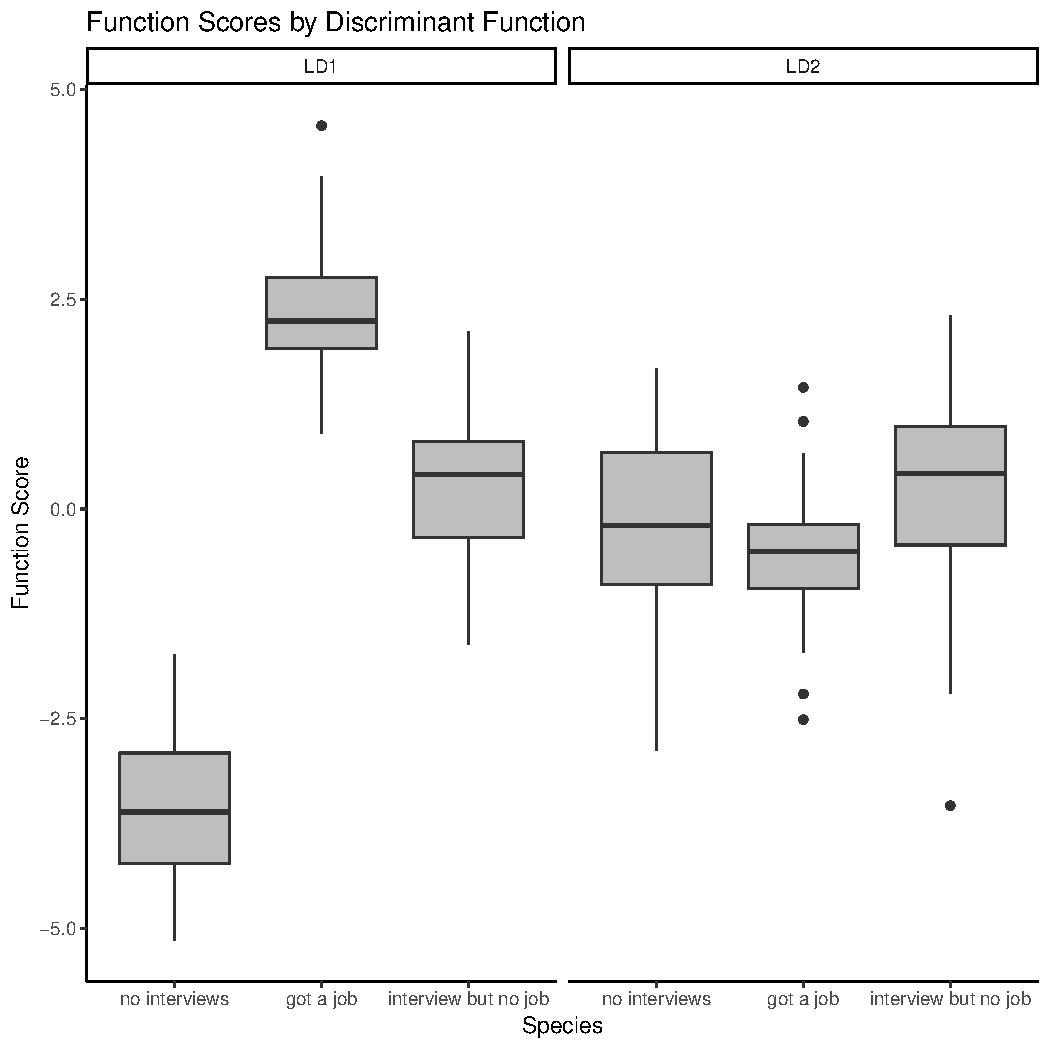
\includegraphics[width=\maxwidth]{figure/unnamed-chunk-5-1} 

\end{knitrout}

Function 1 appears to be discriminating between people who got jobs, interviews, or neither.

\section{Question 4}
How well are the original cases classified?

\subsection{Part A}
Calculate a significance test that compares the classification to what would be expected by chance.

\begin{knitrout}
\definecolor{shadecolor}{rgb}{0.969, 0.969, 0.969}\color{fgcolor}\begin{kframe}
\begin{alltt}
\hlstd{(Class_T} \hlkwb{<-} \hlkwd{table}\hlstd{(}\hlkwc{Original} \hlstd{= dat1}\hlopt{$}\hlstd{outcome,} \hlkwc{Predicted} \hlstd{= LDA_Values}\hlopt{$}\hlstd{class))}
\end{alltt}
\begin{verbatim}
##         Predicted
## Original   1   2   3
##        1  51   0   3
##        2   0  48  23
##        3   2  12 111
\end{verbatim}
\begin{alltt}
\hlcom{# Total observations}
\hlstd{N} \hlkwb{<-} \hlkwd{nrow}\hlstd{(dat1)}

\hlcom{# Observed agreement}
\hlstd{O} \hlkwb{<-} \hlkwd{sum}\hlstd{(}\hlkwd{diag}\hlstd{(Class_T))}

\hlcom{# Marginals (O = Observed, P = Predicted)}
\hlstd{MO1} \hlkwb{<-} \hlstd{MP1} \hlkwb{<-} \hlkwd{sum}\hlstd{(Class_T[}\hlnum{1}\hlstd{, ])}
\hlstd{MO2} \hlkwb{<-} \hlstd{MP2} \hlkwb{<-} \hlkwd{sum}\hlstd{(Class_T[}\hlnum{2}\hlstd{, ])}
\hlstd{MO3} \hlkwb{<-} \hlstd{MP3} \hlkwb{<-} \hlkwd{sum}\hlstd{(Class_T[}\hlnum{3}\hlstd{, ])}

\hlcom{# Expected agreement}
\hlstd{E} \hlkwb{<-} \hlstd{(MO1} \hlopt{*} \hlstd{MP1}\hlopt{/}\hlstd{N)} \hlopt{+} \hlstd{(MO2} \hlopt{*} \hlstd{MP2}\hlopt{/}\hlstd{N)} \hlopt{+} \hlstd{(MO3} \hlopt{*} \hlstd{MP3}\hlopt{/}\hlstd{N)}

\hlstd{t} \hlkwb{<-} \hlstd{(O} \hlopt{-} \hlstd{E)}\hlopt{/}\hlkwd{sqrt}\hlstd{(N} \hlopt{*} \hlstd{(E}\hlopt{/}\hlstd{N)} \hlopt{*} \hlstd{(}\hlnum{1} \hlopt{-} \hlstd{E}\hlopt{/}\hlstd{N))}
\hlstd{t}
\end{alltt}
\begin{verbatim}
## [1] 15.0929
\end{verbatim}
\begin{alltt}
\hlstd{chi_squared} \hlkwb{<-} \hlstd{(((O} \hlopt{-} \hlstd{E)}\hlopt{^}\hlnum{2}\hlstd{)}\hlopt{/}\hlstd{E)} \hlopt{+} \hlstd{((((}\hlnum{250} \hlopt{-} \hlstd{O)} \hlopt{-} \hlstd{(}\hlnum{250} \hlopt{-} \hlstd{E))}\hlopt{^}\hlnum{2}\hlstd{)}\hlopt{/}\hlstd{(}\hlnum{250} \hlopt{-}\hlstd{E))}
\hlstd{chi_squared}
\end{alltt}
\begin{verbatim}
## [1] 227.7956
\end{verbatim}
\end{kframe}
\end{knitrout}

\subsection{Part B}
Calculate Klecka’s tau.

\begin{knitrout}
\definecolor{shadecolor}{rgb}{0.969, 0.969, 0.969}\color{fgcolor}\begin{kframe}
\begin{alltt}
\hlstd{Tau} \hlkwb{<-} \hlstd{(O} \hlopt{-} \hlstd{E)}\hlopt{/}\hlstd{(N} \hlopt{-} \hlstd{E)}
\hlstd{Tau}
\end{alltt}
\begin{verbatim}
## [1] 0.7430495
\end{verbatim}
\end{kframe}
\end{knitrout}

\section{Question 5}
\subsection{Part A}
What is the most common type of misclassification?

\textcolor{blue}{The most common misclassification was for people who were classified as interviewed but not hired who were actually hired.}

\begin{knitrout}
\definecolor{shadecolor}{rgb}{0.969, 0.969, 0.969}\color{fgcolor}\begin{kframe}
\begin{alltt}
\hlstd{plot_data} \hlkwb{<-} \hlkwd{cbind}\hlstd{(LDA_Values}\hlopt{$}\hlstd{x[,} \hlnum{1}\hlstd{], LDA_Values}\hlopt{$}\hlstd{x[,} \hlnum{2}\hlstd{], LDA_Values}\hlopt{$}\hlstd{class, dat1}\hlopt{$}\hlstd{outcome)}
\hlstd{plot_data} \hlkwb{<-} \hlkwd{as.data.frame}\hlstd{(plot_data)}
\hlkwd{names}\hlstd{(plot_data)} \hlkwb{<-} \hlkwd{c}\hlstd{(}\hlstr{"DS1"}\hlstd{,} \hlstr{"DS2"}\hlstd{,} \hlstr{"Class"}\hlstd{,} \hlstr{"Outcome"}\hlstd{)}
\hlstd{plot_data}\hlopt{$}\hlstd{Class_F} \hlkwb{<-} \hlkwd{factor}\hlstd{(plot_data}\hlopt{$}\hlstd{Class,} \hlkwc{levels} \hlstd{=} \hlkwd{c}\hlstd{(}\hlnum{1}\hlstd{,} \hlnum{2}\hlstd{,} \hlnum{3}\hlstd{),} \hlkwc{labels} \hlstd{=} \hlkwd{c}\hlstd{(}\hlstr{"no interviews"}\hlstd{,} \hlstr{"got a job"}\hlstd{,} \hlstr{"interview but no job"}\hlstd{))}
\hlstd{plot_data}\hlopt{$}\hlstd{Outcome_F} \hlkwb{<-} \hlkwd{factor}\hlstd{(plot_data}\hlopt{$}\hlstd{Outcome,} \hlkwc{levels} \hlstd{=} \hlkwd{c}\hlstd{(}\hlnum{1}\hlstd{,} \hlnum{2}\hlstd{,} \hlnum{3}\hlstd{),} \hlkwc{labels} \hlstd{=} \hlkwd{c}\hlstd{(}\hlstr{"no interviews"}\hlstd{,} \hlstr{"got a job"}\hlstd{,} \hlstr{"interview but no job"}\hlstd{))}

\hlkwd{ggplot}\hlstd{(plot_data,} \hlkwd{aes}\hlstd{(}\hlkwc{x} \hlstd{= DS1,} \hlkwc{y} \hlstd{= DS2,} \hlkwc{color} \hlstd{= Class_F))} \hlopt{+}
  \hlkwd{geom_point}\hlstd{(}\hlkwc{shape} \hlstd{=} \hlnum{19}\hlstd{,} \hlkwc{size} \hlstd{=} \hlnum{2}\hlstd{,} \hlkwc{na.rm} \hlstd{=} \hlnum{TRUE}\hlstd{)} \hlopt{+}
  \hlkwd{scale_color_manual}\hlstd{(}\hlkwc{values} \hlstd{=}\hlkwd{c}\hlstd{(}\hlstr{"red"}\hlstd{,} \hlstr{"blue"}\hlstd{,} \hlstr{"green4"}\hlstd{))} \hlopt{+}
  \hlkwd{geom_text}\hlstd{(}\hlkwd{aes}\hlstd{(}\hlkwc{label} \hlstd{= Outcome_F),} \hlkwc{hjust} \hlstd{=} \hlopt{-}\hlnum{.25}\hlstd{,} \hlkwc{vjust} \hlstd{=} \hlnum{0}\hlstd{,} \hlkwc{size} \hlstd{=} \hlnum{2.5}\hlstd{)} \hlopt{+}
  \hlkwd{xlab}\hlstd{(}\hlstr{"Discriminant Function 1"}\hlstd{)} \hlopt{+}
  \hlkwd{ylab}\hlstd{(}\hlstr{"Discriminant Function 2"}\hlstd{)} \hlopt{+}
  \hlkwd{theme_classic}\hlstd{()} \hlopt{+}
  \hlkwd{ggtitle}\hlstd{(}\hlstr{"Discriminant Function Scores by Outcome"}\hlstd{)} \hlopt{+}
  \hlkwd{theme}\hlstd{(}\hlkwc{legend.position} \hlstd{=} \hlstr{"bottom"}\hlstd{)}
\end{alltt}
\end{kframe}
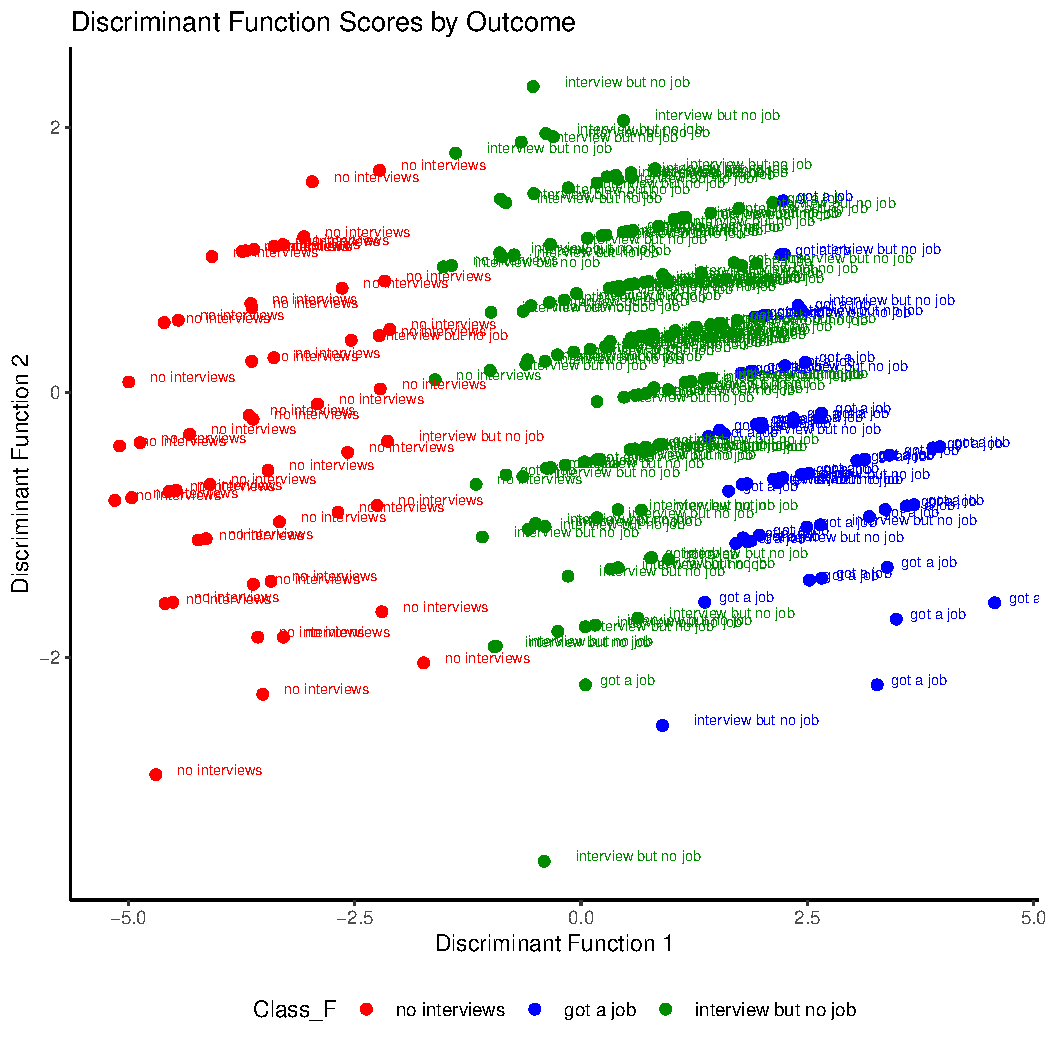
\includegraphics[width=\maxwidth]{figure/unnamed-chunk-8-1} 

\end{knitrout}

\subsection{Part B}
Speculate about what might account for this misclassification?

There are likely a number of additional variables that factor into whether someone gets a job interview or job (or not).

\subsection{Part C}
What additional predictor(s) might this suggest for future analysis? (There is no correct answer here; speculate about what else might determine job search outcome beyond the variables included in the present data.)

Prestige of granting institution, prestige of mentor, conference networking, blog/social media presence, teaching experience

\section{Question 6}
How well are the cases classified using the jackknife (leave-one-out) procedure?

\begin{knitrout}
\definecolor{shadecolor}{rgb}{0.969, 0.969, 0.969}\color{fgcolor}\begin{kframe}
\begin{alltt}
\hlstd{jackknife_1} \hlkwb{<-} \hlkwd{lda}\hlstd{(outcome} \hlopt{~} \hlstd{gre} \hlopt{+} \hlstd{pubs} \hlopt{+} \hlstd{years,} \hlkwc{data} \hlstd{= dat1,} \hlkwc{CV} \hlstd{=} \hlnum{TRUE}\hlstd{)}
\hlstd{Jack_T} \hlkwb{<-} \hlkwd{table}\hlstd{(}\hlkwc{Original} \hlstd{= dat1}\hlopt{$}\hlstd{outcome,} \hlkwc{Predicted} \hlstd{= jackknife_1}\hlopt{$}\hlstd{class)}
\hlstd{Proportion_of_Correct_Classification} \hlkwb{<-} \hlkwd{sum}\hlstd{(}\hlkwd{diag}\hlstd{(Jack_T))}\hlopt{/}\hlkwd{sum}\hlstd{(Jack_T)}
\hlstd{Proportion_of_Correct_Classification}
\end{alltt}
\begin{verbatim}
## [1] 0.836
\end{verbatim}
\end{kframe}
\end{knitrout}

\section{Question 7}
How well are cases in the cross-validation sample classified?

\begin{knitrout}
\definecolor{shadecolor}{rgb}{0.969, 0.969, 0.969}\color{fgcolor}\begin{kframe}
\begin{alltt}
\hlstd{Train_1} \hlkwb{<-} \hlkwd{lda}\hlstd{(outcome} \hlopt{~} \hlstd{gre} \hlopt{+} \hlstd{pubs} \hlopt{+} \hlstd{years,} \hlkwc{data} \hlstd{= dat1,} \hlkwc{CV} \hlstd{=} \hlnum{FALSE}\hlstd{)}

\hlstd{Predict_1} \hlkwb{<-} \hlkwd{predict}\hlstd{(Train_1,} \hlkwc{newdata} \hlstd{= dat2)}

\hlstd{(tab} \hlkwb{<-} \hlkwd{table}\hlstd{(}\hlkwc{Original} \hlstd{= dat2}\hlopt{$}\hlstd{outcome,} \hlkwc{Predicted} \hlstd{= Predict_1}\hlopt{$}\hlstd{class))}
\end{alltt}
\begin{verbatim}
##         Predicted
## Original   1   2   3
##        1  59   0   7
##        2   0  44  21
##        3   3  13 103
\end{verbatim}
\begin{alltt}
\hlkwd{sum}\hlstd{(}\hlkwd{diag}\hlstd{(tab))}\hlopt{/}\hlkwd{sum}\hlstd{(tab)}
\end{alltt}
\begin{verbatim}
## [1] 0.824
\end{verbatim}
\end{kframe}
\end{knitrout}

Decently well (Percent classified correct was 82.4)\%.

\section{Question 8}
Based on the analysis, what advice would you give to a student 
thinking about a career in academia?

\begin{knitrout}
\definecolor{shadecolor}{rgb}{0.969, 0.969, 0.969}\color{fgcolor}\begin{kframe}
\begin{alltt}
\hlstd{dat} \hlopt \hlkwd{gather}\hlstd{(}\hlkwc{key} \hlstd{= item,} \hlkwc{value} \hlstd{= value, gre}\hlopt{:}\hlstd{years)} \hlopt
  \hlkwd{mutate}\hlstd{(}\hlkwc{outcome} \hlstd{=} \hlkwd{mapvalues}\hlstd{(outcome,} \hlkwc{from} \hlstd{=} \hlkwd{c}\hlstd{(}\hlnum{1}\hlstd{,} \hlnum{2}\hlstd{,} \hlnum{3}\hlstd{),} \hlkwc{to} \hlstd{=} \hlkwd{c}\hlstd{(}\hlstr{"no interviews"}\hlstd{,} \hlstr{"got a job"}\hlstd{,} \hlstr{"interview but no job"}\hlstd{)))} \hlopt
  \hlkwd{group_by}\hlstd{(outcome, item)} \hlopt
  \hlkwd{summarize}\hlstd{(}\hlkwc{value} \hlstd{=} \hlkwd{mean}\hlstd{(value,} \hlkwc{na.rm} \hlstd{= T))} \hlopt
  \hlkwd{ggplot}\hlstd{(}\hlkwd{aes}\hlstd{(}\hlkwc{x}\hlstd{=item,} \hlkwc{y} \hlstd{= value,} \hlkwc{fill} \hlstd{= outcome))} \hlopt{+}
    \hlkwd{geom_bar}\hlstd{(}\hlkwc{stat} \hlstd{=} \hlstr{"identity"}\hlstd{,} \hlkwc{position} \hlstd{=} \hlstr{"dodge"}\hlstd{)} \hlopt{+}
    \hlkwd{facet_wrap}\hlstd{(}\hlopt{~}\hlstd{item,} \hlkwc{scale} \hlstd{=} \hlstr{"free"}\hlstd{)} \hlopt{+}
    \hlkwd{theme_classic}\hlstd{()}
\end{alltt}
\end{kframe}
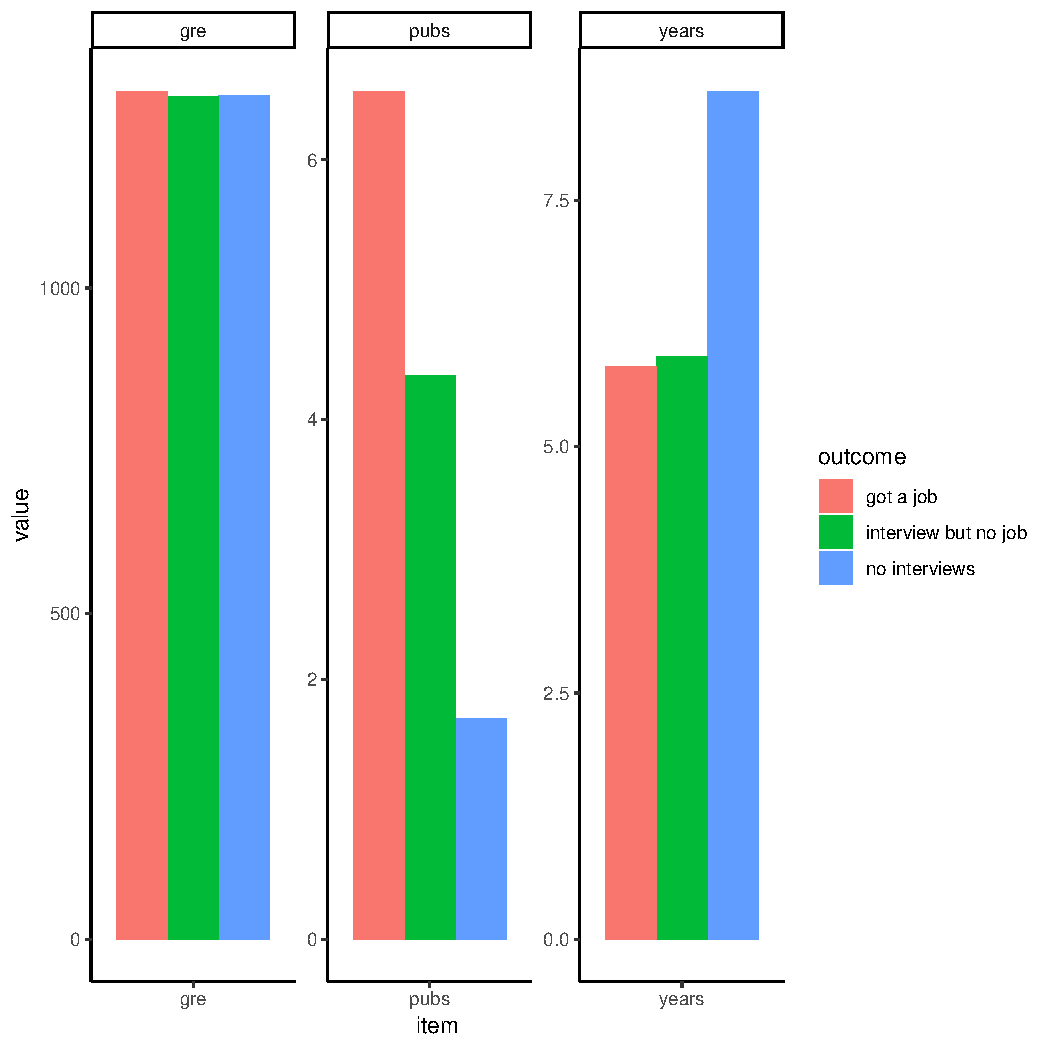
\includegraphics[width=\maxwidth]{figure/unnamed-chunk-11-1} 

\end{knitrout}

Publish or perish. And get out fast. 

\end{document}
